% \iffalse meta-comment
%
% Copyright (C) 2005 by Stephan Hennig <stephanhennig@arcor.de>
% -------------------------------------------------------------
% 
% This file may be distributed and/or modified under the
% conditions of the LaTeX Project Public License, either version 1.2
% of this license or (at your option) any later version.
% The latest version of this license is in:
%
%    http://www.latex-project.org/lppl.txt
%
% and version 1.2 or later is part of all distributions of LaTeX 
% version 1999/12/01 or later.
%
% \fi
%
% \iffalse
%<package>\NeedsTeXFormat{LaTeX2e}[1999/12/01]
%<package>\ProvidesPackage{semioneside}
%<package>  [2005/09/19 v0.41 Put only special contents on left-hand pages (SH)]
%
%<*driver>
\documentclass{ltxdoc}
\usepackage{semioneside}[2005/09/18]\semionesideoff
\usepackage{graphicx}
\usepackage{ifpdf}
\ifpdf
  \DeclareGraphicsRule{*}{mps}{*}{}
\fi
\EnableCrossrefs         
\CodelineIndex
\RecordChanges
\begin{document}
  \DocInput{semioneside.dtx}
  \PrintChanges
  \PrintIndex
\end{document}
%</driver>
% \fi
%
% \CheckSum{61}
%
% \CharacterTable
%  {Upper-case    \A\B\C\D\E\F\G\H\I\J\K\L\M\N\O\P\Q\R\S\T\U\V\W\X\Y\Z
%   Lower-case    \a\b\c\d\e\f\g\h\i\j\k\l\m\n\o\p\q\r\s\t\u\v\w\x\y\z
%   Digits        \0\1\2\3\4\5\6\7\8\9
%   Exclamation   \!     Double quote  \"     Hash (number) \#
%   Dollar        \$     Percent       \%     Ampersand     \&
%   Acute accent  \'     Left paren    \(     Right paren   \)
%   Asterisk      \*     Plus          \+     Comma         \,
%   Minus         \-     Point         \.     Solidus       \/
%   Colon         \:     Semicolon     \;     Less than     \<
%   Equals        \=     Greater than  \>     Question mark \?
%   Commercial at \@     Left bracket  \[     Backslash     \\
%   Right bracket \]     Circumflex    \^     Underscore    \_
%   Grave accent  \`     Left brace    \{     Vertical bar  \|
%   Right brace   \}     Tilde         \~}
%
%
% \changes{v0.4}{2005/07/30}{.dtx package version with revised
% documentation}
% \changes{v0.41}{2005/09/19}{included MetaPost source in .dtx file}
% \changes{v0.41}{2005/09/19}{released package on CTAN}
%
% \GetFileInfo{semioneside.sty}
%
% \DoNotIndex{\newcommand,\newenvironment,\ifx,\fi,\global,\let}
% 
%
% \title{The \textsf{semioneside} package\thanks{This document
%   corresponds to \textsf{semioneside}~\fileversion, dated
%   \filedate.}}
% \author{Stephan Hennig\\ \texttt{stephanhennig@arcor.de}}
%
% \maketitle
%
% \begin{abstract}
% This package supports the creation of semi one sided documents.
% That is, two sided documents, where all text is output on
% right-hand pages---like in one sided documents---and only special
% contents is output on left-hand pages on user request,
% \emph{e.\,g.}, floating elements.
% \end{abstract}
%
%
% \section{Introduction}
%
% Some institutions require a document layout where running text
% appears on right-hand pages only---as in one sided documents---,
% but figures and tables, and only those, are displayed on left-hand
% pages. This package supports the preparation of such semi one
% sided documents. That is, all running text is output on
% right-hand pages and only special content, \emph{e.\,g.},
% floating objects, are output on left-hand pages on user request.
% Otherwise left-hand pages stay empty.
%
% References to left-hand pages are possible by defining a proper
% label on a left-hand page. The page counter can be configured to:
% \begin{itemize}
% \item keep left-hand pages syncronized with the facing right-hand
% page,
% \item keep left-hand pages syncronized with the preceeding
% right-hand page, \emph{i.\,e.}, page numbers refer to single
% sheets, or
% \item count every left- and right-hand page as in normal two
% sided documents.
% \end{itemize}
%
% \emph{When using this package keep in mind that this is more a
% quick hack than a robust solution!} Several problems are listed
% in section \ref{sec:knownproblems}.\footnote{The best solution to
% avoid all sorts of problems is not to use this package. You have
% been warned!}
%
%
% \section{How It Works}
%
% Before describing the usage of the \textsf{semioneside} package
% lets have a look at how it works behind the scenes.
%
% The functionality of the \textsf{semioneside} package is based on
% the |\afterpage| macro from the |afterpage| package. What happens
% after a page break is essentially this:
% \begin{enumerate}
% \item Since the current page break happend to occur at the end of
% a right-hand page---remember that the first page of a document is
% a right-hand page---, a new left-hand page begins. Now the
% |afterpage| package calls the working macro
% |\semioneside@skipleftpage| which in turn calls these macros:
% \begin{verbatim}
%\leftpagecontrolstart
%\leftpagecontent
%\leftpagecontrolend
%\clearpage
%\rightpagecontrolstart
% \end{verbatim}
%
% \item The |\clearpage| command in the macro sequence above
% finishes the left-hand page and so macro |\rightpagecontrolstart|
% is called at the beginning of a new right-hand page.
%
% \item Now, everything is ready to continue running text from the
% last right-hand page. At the next page break again |afterpage|
% calls |\semioneside@skipleftpage| and steps~1 to~3 are repeated.
% \end{enumerate}
% The complete procedure is illustrated in
% Figure~\ref{fig:procedure}.
% \begin{figure}[t]
%   \centering
%   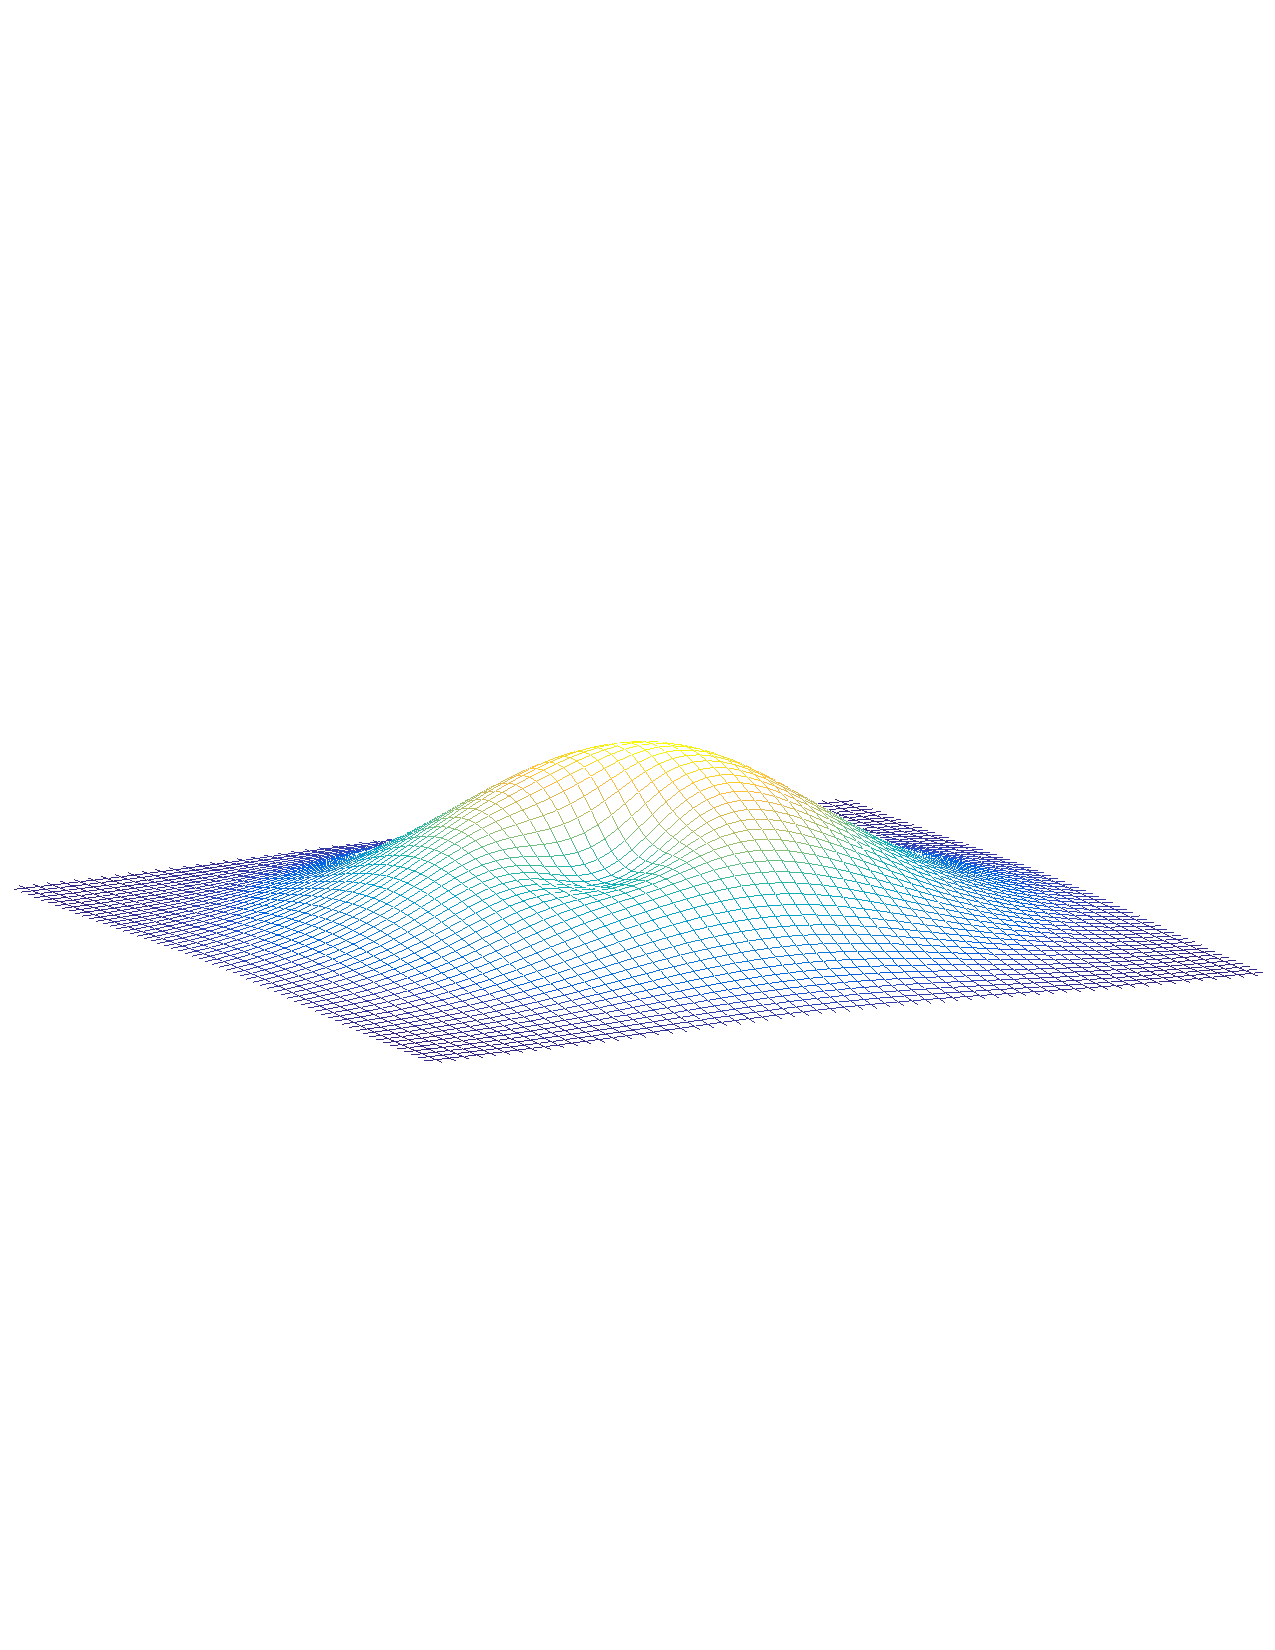
\includegraphics{figure.1}
%   \caption{How the \textsf{semioneside} package intercepts page
%   breaks.}
%   \label{fig:procedure}
% \end{figure}
%
%
% \section{Usage}
%
% As can be seen, four macros are called during type setting left-
% and right-hand pages. Macro
% |\leftpagecontent|\DescribeMacro{\leftpagecontent}{} is the main
% user macro. It contains the stuff that shall be output on the
% next left-hand page and can be modified via |\renewcommand|. If
% you want to have a figure on a left-hand page you should pass the
% whole figure environment including caption and label to
% |\leftpagecontent| (see the example code in file |example.tex|).
%
% The remaining three macros
% |\leftpagecontrolstart|\DescribeMacro{\leftpagecontrolstart},
% |\leftpagecontrolend|\DescribeMacro{\leftpagecontrolend}{} and
% |\rightpagecontrolstart|\DescribeMacro{\rightpagecontrolstart}{}
% are hooks and can be used to adjust page numbering, the page
% style of left-hand pages \emph{etc}. By default
% |\leftpagecontrolstart| calls |\thispagestyle{empty}|, macro
% |\leftpagecontrolend| is empty and macro |\rightpagecontrolstart|
% decreases the page counter by one. That is, left-hand pages have
% no head and foot line and the page number equals that of the
% facing right-hand page. Note, the page counter is not adjusted on
% a left-hand page, but on the following right-hand page.
%
% Issuing the following macro sequence in the document preamble
% results in a layout where left-hand pages have the same page
% number as the preceeding right-hand page, \emph{i.\,e.}, page
% numbers refer to sheets. Additionally page numbers are shown on
% left-hand pages:
% \begin{verbatim}
%\renewcommand*{\leftpagecontrolstart}{%
%  \pagestyle{plain}%
%  \addtocounter{page}{-1}%
%}
%\renewcommand*{\leftpagecontrolend}{}
%\renewcommand*{\rightpagecontrolstart}{}
% \end{verbatim}
%
% There are two more user macros,
% |\semionesideoff|\DescribeMacro{\semionesideoff}{} and
% |\semionesideon|\DescribeMacro{\semionesideon}{}, which can be used
% to turn semi one sided layout off and on manually in the document.
% You might have to insert an empty page manually before
% |\semionesideon| to keep left- and right-hand pages syncronized.
% By default, semi one sided layout is activated.
%
%
% \section{Known Problems}\label{sec:knownproblems}
%
% Since this package is everything but a robust solution, there are
% some issues you have to take care of:
% \begin{enumerate}
% \item Contents that shall be output on a left-hand page has to be
% declared \emph{on the preceeding} right-hand page. Since there is
% only a narrow window of approx. one page to declare left-hand
% page contents, it is recommended to finish running text first and
% only deal with left-hand page contents when page breaks of the
% document are stable.
%
% \item Paragraphs longer than one page can cause the whole
% mechanism to get out-of-sync. This seems to be due to \TeX's page
% breaking mechanism. When a paragraph breaks across several pages
% the |\afterpage| command is not executed at a page break (at
% least not reliably) and all gets mixed up. Beware of too long
% paragraphs!
%
% \item\label{enum:book} When using document class |book| a blank
% page seems to be inserted before the first |\chapter| or
% |\maketitle| command. A workaround is to call macro
% |\semionesideoff| directly after loading the package in the
% document preamble and call macro |\semionesideon| manually after
% |\maketitle| or the first |\chapter| command. See also the next
% issue.
%
% \item\label{enum:memoir} A similar problem was reported with the
% |memoir| class and |\part| command, which inserts two empty pages
% instead of only one. A workaround was to copy |memoir|'s
% definition of |\part| and remove a |\newpage| call there. In case
% you call this dirty hacking, you have been warned before.
%
% \item When switching semi one sided layout on and off manually in
% the document pages can get out-of-sync. To avoid this, try to add
% a |\clearpage| or |\cleardoublepage| command before
% |\semionesideon|. If pages are still out-of- sync try to add the
% following macro sequence:
% \begin{verbatim}
%\clear(double)page
%\leftpagecontrolstart\null\leftpagecontrolend
%\clearpage
%\rightpagecontrolstart
% \end{verbatim}
%
% \item At the end of the document one or two empty pages may be
% appended. To get rid of those just call |\semionesideoff| before
% |\end{document}|.
% \end{enumerate}
%
% I'm sure there are a lot more problems one can run into. In case
% you can't solve them by hand, try to set your document without
% the \textsf{semioneside} package and present this to your editor
% or boss for approval.\footnote{Don't tell them the rules are bad.
% Just asking if the document is ok, might be the better way.}
% Since figures on left-hand pages were originally meant as a help
% when preparing manuscripts on type writers, there is no real
% benefit in it in digital document preparation.
%
%
% \section{Tips \& Tricks}
%
% \paragraph{Symmetric and asymmetric type area}
% This package works with the
% standard classes |article|, |report| and |book|. The |article|
% class leads to a symmetric layout. You can get a symmetric
% layout with the |report| or |book| classes, too, by calling them
% with the |oneside| document class option (see
% issue~\ref{enum:book} in section~\ref{sec:knownproblems}).
% Omitting this option unfortunately leads to an alternating type
% area on right-hand pages. (I don't know why.) In case you need an
% asymmetric layout with the |book| class have a look at the
% |asymmetric| option of the |geometry| package.
%
%
% \section{Bugs and Development}
%
% As mentioned before, this package is no perfect solution to the
% problem it tries to solve, but rather a quick shot. Since I
% don't think I can improve on it much, I would appreciate if
% someone would take over development or rewrite this package from
% scratch to make the code more robust.
%
% Anyway, if you find bugs (and hopefully workarounds) feel free
% to contact me at \texttt{stephanhennig@arcor.de}. I'll try to
% list them in the \emph{Known Problems} section at least.
%
% \iffalse
%<*figure>
verbatimtex
\documentclass{article}
\begin{document}
\footnotesize
etex
prologues := 1;
beginfig(1);
  numeric pwd, pht, pdx;
  pwd = 110bp;
  pht = 110bp;
  pdy = .1*pht;
  spht = .6pht;
  
  pickup pencircle scaled .8bp;
  draw ( (0bp,0bp)--(2pwd,0bp)--(2pwd,spht)..{dir 190}(pwd,spht)..(0bp,spht)--cycle ) shifted (0bp,pht+pdy);
  draw ( (pwd,0bp)--(pwd,spht) ) shifted (0bp,pht+pdy);
  draw unitsquare xscaled 2pwd yscaled pht;
  draw (pwd,0bp)--(pwd,pht);
  draw ( (0bp,0bp)--(2pwd,0bp)--(2pwd,-spht)..{dir 190}(pwd,-spht)..(0bp,-spht)--cycle ) shifted (0bp,-pdy);
  draw ( (pwd,0bp)--(pwd,-spht) ) shifted (0bp,-pdy);
  
  label.top(btex left hand page etex, (.5pwd,spht) shifted (0bp,pht+2pdy));
  label.top(btex right hand page etex, (1.5pwd,spht) shifted (0bp,pht+2pdy));
  label.top(btex \parbox{100pt}{\itshape\dotfill\ running text \dotfill} etex, (1.5pwd,0bp) shifted (0bp,pht+pdy));
  label.rt(btex \begin{tabular}{@{}l@{}}page\\break\end{tabular} etex, (2pwd,0bp) shifted (.5pdy,pht+pdy));
  label.llft(btex \begin{tabular}[c]{@{}l@{}}called via\\\texttt{\textbackslash afterpage}\end{tabular} $\left\{\mathrm{\raisebox{-2\baselineskip}{\rule{0pt}{4\baselineskip}}}\right.$  etex, (0bp,pht) shifted (-.25pdy,0bp));
  label.bot(btex \parbox{100pt}{\ttfamily\textbackslash leftpagecontrolstart\par\textbackslash leftpagecontent\par\textbackslash leftpagecontrolend\par\textbackslash clearpage} etex, (.5pwd,pht));
  label.bot(btex \parbox{100pt}{\texttt{\textbackslash rightpagecontrolstart}\par\dotfill\ \textit{running text} \dotfill} etex, (1.5pwd,pht));
  label.top(btex \parbox{100pt}{\itshape\dotfill\ running text \dotfill} etex, (1.5pwd,0bp));
  label.rt(btex \begin{tabular}{@{}l@{}}page\\break\end{tabular} etex, (2pwd,0bp) shifted (.5pdy,0bp));
  label.llft(btex \begin{tabular}[c]{@{}l@{}}called via\\\texttt{\textbackslash afterpage}\end{tabular} $\left\{\mathrm{\raisebox{-2\baselineskip}{\rule{0pt}{4\baselineskip}}}\right.$ etex, (0bp,-pdy) shifted (-.25pdy,0bp));
  label.bot(btex \parbox{100pt}{\ttfamily\textbackslash leftpagecontrolstart\par\textbackslash leftpagecontent\par\textbackslash leftpagecontrolend\par\textbackslash clearpage} etex, (.5pwd,-pdy));
  label.bot(btex \parbox{100pt}{\texttt{\textbackslash rightpagecontrolstart}\par\dotfill\ \textit{running text} \dotfill} etex, (1.5pwd,-pdy));
  
  pickup pencircle scaled .4bp;
  drawarrow (.25pwd,pht-45pt){dir -45}..(.8pwd,pht-30pt)..{right}(.99pwd,.95pht);
  drawarrow ( (.25pwd,pht-45pt){dir -45}..(.8pwd,pht-30pt)..{right}(.99pwd,.95pht) ) shifted (0bp,-pht-pdy);
endfig;

end
%</figure>
% \fi
%
% \iffalse
%<*example>
\documentclass{article}
\usepackage{semioneside}
\usepackage[english]{babel}
\usepackage{blindtext}
\begin{document}
\section{Example}
\Blindtext[3]
\renewcommand{\leftpagecontent}{
 \begin{figure}
   \centering
   \rule{4cm}{2cm}
   \caption{A picture.}
   \label{fig:picA}
 \end{figure}
}
\Blindtext[3]
A reference to figure~\ref{fig:picB} on p.~\pageref{fig:picB}.
\renewcommand{\leftpagecontent}{
 \begin{figure}
   \centering
   \rule{3cm}{2cm}
   \caption{A second picture.}
   \label{fig:picB}
 \end{figure}
 \begin{figure}
   \centering
   \rule{4cm}{5cm}
   \caption{A third picture.}
   \label{fig:picC}
 \end{figure}
}
\Blindtext[6]
A reference to figure~\ref{fig:picA} on p.~\pageref{fig:picA}
\semionesideoff
\end{document}
%</example>
% \fi
%
%
% \StopEventually{\PrintChanges}
%
%
%<*package>
% \section{Implementation}
%
% Make sure the |afterpage| package is loaded.
%    \begin{macrocode}
\RequirePackage{afterpage}
%    \end{macrocode}
%
% \begin{macro}{\leftpagecontent}
% Define a macro that stores the contents that shall be output on
% a left-hand page.
%    \begin{macrocode}
\newcommand*{\leftpagecontent}{}
%    \end{macrocode}
% \end{macro}
%
% \begin{macro}{\leftpagecontrolstart}
% Define a macro that may contain control statements that are
% executed at the beginning of left-hand pages before
% |\leftpagecontent|. Default is to make the left-hand page
% style |empty| here.
%    \begin{macrocode}
\newcommand*{\leftpagecontrolstart}{%
  \thispagestyle{empty}%
}
%    \end{macrocode}
% \end{macro}
%
% \begin{macro}{\leftpagecontrolend}
% Define a macro that may contain control statements that are
% executed at the end of left-hand pages after |\leftpagecontent|.
% By default, it is empty.
%    \begin{macrocode}
\newcommand*{\leftpagecontrolend}{}
%    \end{macrocode}
% \end{macro}
%
% \begin{macro}{\rightpagecontrolstart}
% Define a macro that may contain control statements that are
% executed at the beginning of right-hand pages before the running
% text continues. By default, the page counter is decreased by one
% here.
%    \begin{macrocode}
\newcommand*{\rightpagecontrolstart}{%
  \addtocounter{page}{-1}%
}
%    \end{macrocode}
% \end{macro}
%
% \begin{macro}{\semioneside@longempty}
% Define a long \emph{empty} macro which is used in a test (see
% |\ifx| below).
%    \begin{macrocode}
\newcommand*{\semioneside@longempty}{}
%    \end{macrocode}
% \end{macro}
%
% \begin{macro}{\semioneside@skipleftpage}
% This is the working macro. It calls itself recursively via
% |\afterpage|. The recursion can be started by issuing the command
% |\semionesideon|. In fact, this is already done when the package
% is loaded.
%    \begin{macrocode}
\newcommand*{\semioneside@skipleftpage}{}
%    \end{macrocode}
% \end{macro}
%
% \begin{macro}{\semioneside@skipleftpagetemplate}
% Define a template for the working macro
% |\semioneside@skipleftpage|. This is used in |\semionesideon|.
%    \begin{macrocode}
\newcommand*{\semioneside@skipleftpagetemplate}{%
  \ifx\leftpagecontent\empty%
    \let\leftpagecontent\null%
  \fi%
  \ifx\leftpagecontent\semioneside@longempty%
    \let\leftpagecontent\null%
  \fi%
  \leftpagecontrolstart%
  \leftpagecontent%
  \leftpagecontrolend%
  \clearpage%
  \rightpagecontrolstart%
  \afterpage{\semioneside@skipleftpage}%
  \global\let\leftpagecontent\empty%
}
%    \end{macrocode}
% \end{macro}
%
% \begin{macro}{\semionesideon}
% Define a macro to activate semi one sided layout.
%    \begin{macrocode}
\newcommand*{\semionesideon}{%
  \global\let\semioneside@skipleftpage\semioneside@skipleftpagetemplate%
  \afterpage{\semioneside@skipleftpage}%
}
%    \end{macrocode}
% \end{macro}
%
% \begin{macro}{\semionesideoff}
% Define a macro to deactivate semi one sided layout.
%    \begin{macrocode}
\newcommand*{\semionesideoff}{%
  \global\let\semioneside@skipleftpage\empty%
  \global\let\leftpagecontent\empty%
}
%    \end{macrocode}
% \end{macro}
%
% Switch on semi one sided layout.
%    \begin{macrocode}
\semionesideon
%    \end{macrocode}
%
%</package>
%
% \Finale
